\begin{figure}[!ht]
\centering
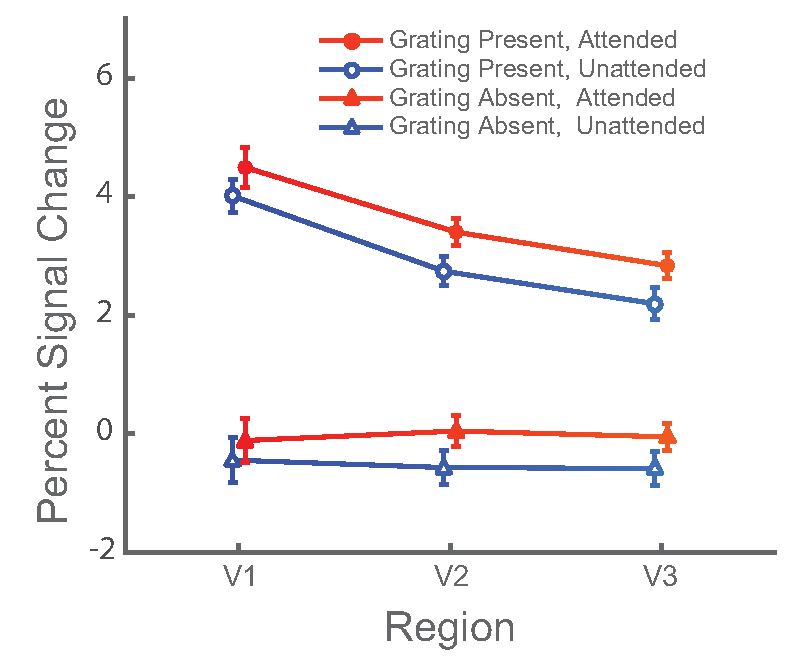
\includegraphics[width=0.8\textwidth, clip=true]{./Chapters/04_Attention/Images/RoiResults}
\caption{Amplitude of the BOLD response for attended and unattended regions in areas V1-V3. Red lines indicate the attended condition, blue the unattended. The top lines (circles) show the response when a grating was presented, the bottom lines (triangles) when no grating was presented, at the attended or unattended location. Response amplitudes were significantly higher for attended than unattended locations and stimuli. Error bars indicate $\pm$1 SEM.}
\label{fig:roiresults}
\end{figure}